\documentclass[a4paper,11pt]{article}

\usepackage{amsmath}
\usepackage[pdftex]{graphicx}

\usepackage[english,greek]{babel}

\usepackage{lmodern}

\usepackage{listings}

\lstset{
  basicstyle=\ttfamily,
  columns=fullflexible,
  frame=single,
  breaklines=true
}

% Αφαίρεσε (Εισήγαγε) την παρακάτω γραμμή σε σχόλιο αν ο επεξεργαστής κειμένου (δεν) χρησιμοποιεί κωδικοποίηση Unicode για Ελληνικά
\usepackage[utf8x]{inputenc}

% Αφαίρεσε (Εισήγαγε) την παρακάτω γραμμή σε σχόλιο αν ο επεξεργαστής κειμένου (δεν) χρησιμοποιεί κωδικοποίηση iso-8859-7 για Ελληνικά
%\usepackage[iso-8859-7]{inputenc}

%Δημιουργία συντομεύσεων για αλλαγή γραφής σε Ελληνικά/Αγγλικά
\newcommand{\lt}{\latintext}
\newcommand{\gt}{\greektext}

\title{2η Υποχρεωτική Εργασία \\ Στο Μάθημα της Αριθμητικής Ανάλυσης: \\ Άσκηση 7}
\author{Ονοματεπώνυμο: Μπαρακλιλής Ιωάννης  \\  ΑΕΜ: 3685}
\date{4 Ιανουαρίου 2021}

\begin{document}

\maketitle
\section{Επιλογή εταιριών μετοχών}
Ως εταιρίες μετοχών επιλέγω τις εταιρίες Ελλάδος (Τράπεζα της-), με σύμβολο ΕΛΛ, και την ΕΛΙΝΟΪΛ ΕΛΛΗΝΙΚΗ ΕΤΑΙΡΙΑ ΠΕΤΡΕΛΑΙΩΝ Α.Ε., με σύμβολο ΕΛΙΝ. Η ημέρα των γενεθλίων μου στο 2020 ήταν στις 2 Οκτωβρίου, επομένως πρέπει να προσεγγίσω την τιμή της κάθε μετοχής στην κοντινότερη στις 2 Οκτωβρίου τιμή κλεισίματος, του χρηματιστηρίου που ήταν στις 5 Οκτωβρίου, με βάση τις προηγούμενες 10 τιμές κλεισίματος. Επίσης, η 5η συνεδρίαση μετά από εκείνη των γενεθλίων  γίνεται στις 09/10/2020\\

\par
Για την μετοχή με σύμβολο ΕΛΛ έχω τιμές κλεισίματος:
\begin{itemize}
    \item Στο κλείσιμο του χρηματιστηρίου στις 18/9/2020 έχω τιμή μετοχής 13,5600
    \item Στο κλείσιμο του χρηματιστηρίου στις 21/9/2020 έχω τιμή μετοχής 13,1600
    \item Στο κλείσιμο του χρηματιστηρίου στις 22/9/2020 έχω τιμή μετοχής 13,4000
    \item Στο κλείσιμο του χρηματιστηρίου στις 23/9/2020 έχω τιμή μετοχής 13,3400
    \item Στο κλείσιμο του χρηματιστηρίου στις 24/9/2020 έχω τιμή μετοχής 13,2800
    \item Στο κλείσιμο του χρηματιστηρίου στις 25/9/2020 έχω τιμή μετοχής 13,3600
    \item Στο κλείσιμο του χρηματιστηρίου στις 28/9/2020 έχω τιμή μετοχής 13,1400
    \item Στο κλείσιμο του χρηματιστηρίου στις 29/9/2020 έχω τιμή μετοχής 13,2200
    \item Στο κλείσιμο του χρηματιστηρίου στις 30/9/2020 έχω τιμή μετοχής 13,0000
    \item Στο κλείσιμο του χρηματιστηρίου στις 1/10/2020 έχω τιμή μετοχής 13,2000
\end{itemize}
Τέλος, στο κλείσιμο στις 5/10/2020, που θέλω να προσεγγίσω, έχω τιμή μετοχής  13,3000

\par
Για την μετοχή με σύμβολο ΕΛΙΝ έχω τιμές κλεισίματος:
\begin{itemize}
    \item Στο κλείσιμο του χρηματιστηρίου στις 18/9/2020 έχω τιμή μετοχής 1,4500
    \item Στο κλείσιμο του χρηματιστηρίου στις 21/9/2020 έχω τιμή μετοχής 1,4500
    \item Στο κλείσιμο του χρηματιστηρίου στις 22/9/2020 έχω τιμή μετοχής 1,5100
    \item Στο κλείσιμο του χρηματιστηρίου στις 23/9/2020 έχω τιμή μετοχής 1,4100
    \item Στο κλείσιμο του χρηματιστηρίου στις 24/9/2020 έχω τιμή μετοχής 1,3700
    \item Στο κλείσιμο του χρηματιστηρίου στις 25/9/2020 έχω τιμή μετοχής 1,3700
    \item Στο κλείσιμο του χρηματιστηρίου στις 28/9/2020 έχω τιμή μετοχής 1,4100
    \item Στο κλείσιμο του χρηματιστηρίου στις 29/9/2020 έχω τιμή μετοχής 1,4100
    \item Στο κλείσιμο του χρηματιστηρίου στις 30/9/2020 έχω τιμή μετοχής 1,4100
    \item Στο κλείσιμο του χρηματιστηρίου στις 1/10/2020 έχω τιμή μετοχής 1,4700
\end{itemize}
Τέλος, στο κλείσιμο στις 5/10/2020, που θέλω να προσεγγίσω, έχω τιμή μετοχής  1,4300

\section{Υλοποίηση}
Το ζητούμενο υλοποιείται προγραμματιστικά στην γλώσσα {\lt python} (3.7) στο αρχείο με όνομα {\lt stock\textunderscore approximation.py} το οποίο φαίνεται παρακάτω:
\lt
\lstinputlisting[language=Python]{stock_approximation.py}
\gt

\par
Στον παραπάνω κώδικα:\\
Αρχικά, ορίζονται οι συναρτήσεις {\lt least\textunderscore squares}, {\lt approximate\textunderscore function\textunderscore with\textunderscore least\textunderscore squares}, {\lt calculate\textunderscore polynomial}, {\lt matrix\textunderscore multiplication}, {\lt matrix\textunderscore transposition}, {\lt swap\textunderscore rows, pivot\textunderscore matrix, matrix\textunderscore vector\textunderscore multiplication, PLU, solve\textunderscore system} οι οποίες συνολικά επιτρέπουν την προσέγγιση ελαχίστων τετραγώνων με πολυώνυμο μίας συνάρτησης  με βάση έναν αριθμό σημείων μίας συνάρτησης χρησιμοποιώντας την συνάρτηση  {\lt approximate\textunderscore function\textunderscore with\textunderscore least\textunderscore squares}. Οι συναρτήσεις αυτές, είναι πανομοιότυπες με εκείνες, με το ίδιο όνομα, που χρησιμοποιήθηκαν για την προσέγγιση του ημίτονου με ελάχιστα τετράγωνα στην άσκηση 5 της 2ης υποχρεωτικής εργασίας οπότε ο ορισμός τους και η αναλυτική περιγραφής τους παραλείπεται. 

\par
Παρ' όλα αυτά είναι χρήσιμο να υπάρχουν οι ορισμοί των συναρτήσεων {\lt approximate\textunderscore function\textunderscore with\textunderscore least\textunderscore squares} και {\lt calculate\textunderscore polynomial} τις οποίες χρησιμοποιούμε άμεσα στο εκτελέσιμο τμήμα του κώδικα:
\par
Η  {\lt approximate\textunderscore function\textunderscore with\textunderscore least\textunderscore squares} δέχεται ως όρισμα έναν δισδιάστο πίνακα όπου η κάθε γραμμή του αποτελεί ένα σημείο όπου στην πρώτη στήλη υπάρχει το {\lt $x$} και στην άλλη το {\lt $y$}, και την τάξη του πολυωνύμου και επιστρέφει έναν μονοδιάστατο πίνακα με τους συντελεστές του πολυωνύμου ίδιας τάξης με αυτή που δόθηκε στο όρισμα που αποτελεί την προσέγγιση με ελάχιστα τετράγωνα. Tο κάθε στοιχείο που περιέχει ο πίνακας αυτός (που επιστρέφεται) αποτελεί τον συντελεστή στην αντίστοιχή θέση (δηλαδή το πρώτο στοιχείο (θέση 0) του πίνακα αντιστοιχεί στην σταθερά, το δεύτερο (θέση 1) αντιστοιχεί στον συντελεστή του {\lt $x$}, το τρίτο (θέση 2), εφόσον το πολυώνυμο είναι δευτέρου βαθμού στον συντελεστή του {\lt $x^2$}, κ.ο.κ.
\par
H {\lt calculate\textunderscore polynomial} δέχεται έναν πίνακα συντελεστών πολυωνύμου (όπου η θέση κάθε στοιχείου αντιστοιχεί στην δύναμη του αγνώστου) και έναν (πραγματικό) αριθμό {\lt x} και υπολογίζει και επιστρέφει την τιμή του πολυωνύμου για το δοθέν σημείο.\\

\par
Τέλος, ορίζεται η συνάρτηση {\lt main}, που δεν δέχεται ορίσματα, η οποία χρησιμοποιεί τις συναρτήσεις {\lt approximate\textunderscore function\textunderscore with\textunderscore least\textunderscore squares} και {\lt calculate\textunderscore polynomial} για να υπολογίσει τις προσεγγίσεις που ζητούνται απο την άσκηση:\\

Αρχικά, ορίζει τον πίνακα {\lt ELL\textunderscore stock} ο οποίος περιέχει την τιμή της μετοχής (ΕΛΛ) σε κάθε συνεδρίαση και τον αριθμό της συνεδρίασης και είναι ένα πίνακας με 10 γραμμές (κάθε γραμμή αντιστοιχεί σε μία μέρα κλεισίματος χρηματιστηρίου) και 2 στήλες. Στην πρώτη στήλη βρίσκεται το σημείο (του πολυωνύμου προσέγγισης που θα προκύψει αργότερα) που αντιστοιχεί στην τιμή μετοχής μίας μέρας κλεισίματος χρηματιστηρίου (η τιμή αυτή αντιστοιχεί στο πόσες συνεδριάσεις  χρηματιστηρίου έχουν περάσει από την πρώτη μέρα των δεδομένων που έχω. Δηλαδή, στην πρώτη συνεδρίαση (στις 18/9/2020) έχω τιμή 0 στην δεύτερη (στις 19/9/2020) έχω 1, κ.ο.κ. για τις υπόλοιπες τιμές). Στην δεύτερη στήλη, υπάρχει η τιμή της μετοχής στον αντίστοιχο αριθμό συνεδρίασης.\\

Στην συνέχεια ορίζεται ο πίνακας {\lt ELL\textunderscore stock\textunderscore dates} ο οποίος περιέχει την ημερομηνία συνεδρίασης που αντιστοιχεί στην κάθε τιμή κλεισίματος και έχει 10 γραμμές (κάθε γραμμή αντιστοιχεί σε μία μέρα κλεισίματος χρηματιστηρίου) και 3 στήλες. Στην πρώτη στήλη βρίσκεται η ημέρα, στην δεύτερη ο μήνας και στην τρίτη ο χρόνος, που αντιστοιχούν στην ημερομηνία κάθε συνεδρίασης.\\

Μετά, προσεγγίζεται η συνάρτηση που δίνει τις τιμές των μετοχών σε κάθε συνεδρίαση με πολυώνυμο 2ου βαθμού (το οποίο αργότερα εμφανίζεται) με προσέγγιση ελαχίστων τετραγώνων με την χρήση της συνάρτησης {\lt approximate\textunderscore function\textunderscore with\textunderscore least\textunderscore squares} που δίνω ως όρισμα τα σημεία που ορίζονται από τον πίνακα {\lt ELL\textunderscore stock} και 2 εφόσον θέλω προσέγγιση με πολυώνουμο 2ου βαθμού και αποθηκεύω το αποτέλεσμα, δηλαδή τους συντελεστές του πολυωνύμου 2ου βαθμού, και αρχικοποιώ την τιμή {\lt max\textunderscore absolute\textunderscore prediction\textunderscore error}, που θα αποθηκεύει την τιμή του μέγιστου απόλυτου σφάλματος των προσεγγίσεων των δεδομένων τιμών, σε -1 (ώστε αργότερα να ανατραπεί εφόσον το απόλυτο σφάλμα είναι μη αρνητικό).\\

Στην συνέχεια, για κάθε ένα σημείο του πίνακα {\lt ELL\textunderscore stock}, δηλαδή για κάθε μία τιμή μετοχής από τα δεδομένα, υπολογίζω και αποθηκεύω την προσέγγιση τιμής μετοχής σε κάθε συνεδρίαση χρησιμοποιώντας την συνάρτηση {\lt calculate\textunderscore polynomial}, με ορίσματα τις τιμές των συντελεστών του πολυωνύμου 2ου βαθμού που αποθήκευσα παραπάνω και το σημείο που αντιστοιχεί στην συνεδρίαση, υπολογίζω και αποθηκεύω το απόλυτο σφάλμα για την προσέγγιση της τιμής αυτής της συνεδρίασης και ενημερώνω (αν χρειάζεται) το μέγιστο απόλυτο σφάλμα και τέλος, εμφανίζω στην οθόνη την ημερομηνία της συνεδρίασης, την προσέγγιση/πρόβλεψη της τιμής μετοχής, την αναμενόμενη (πραγματική) τιμή και το απόλυτο σφάλμα που αποθήκευσα προηγουμένως.\\
Τέλος, αφού υπολογίσω και εμφανίσω τα παραπάνω για κάθε συνεδρίαση, εμφανίζω την τιμή του μέγιστου απολύτου σφάλματος.\\

Ακολούθως, υπολογίζω και εμφανίζω την πρόβλεψη για την τιμή μετοχής συνεδρίασης ημέρας κοντινότερης εκείνης των γενεθλίων μου (που γίνεται στις 5/10/2020) χρησιμοποιώντας την συνάρτηση {\lt calculate\textunderscore polynomial}, με ορίσματα τις τιμές των συντελεστών του πολυωνύμου 2ου βαθμού που αποθήκευσα παραπάνω και το σημείο που αντιστοιχεί στην συνεδρίαση (που εδώ είναι 11, εφόσον είναι η μέρα των γενεθλίων είναι η 10η συνεδρίαση μετά την πρώτη των δεδομένων και η κοντινότερη αυτής της μέρας των γενεθλίων είναι η αμέσως επόμενη δηλαδή η 11η στις 5/10) και εμφανίζω στην οθόνη την ημερομηνία της συνεδρίασης, την προσέγγιση/πρόβλεψη της τιμής μετοχής, την αναμενόμενη (πραγματική) τιμή (που γνωρίζω ότι είναι 13,3000) και το απόλυτο σφάλμα της πρόβλεψης.\\

Τέλος, προσεγγίζω (χρησιμοποιώντας την συνάρτηση {\lt calculate\textunderscore polynomial}, με ορίσματα τις τιμές των συντελεστών του πολυωνύμου 2ου βαθμού που αποθήκευσα παραπάνω και το σημείο που αντιστοιχεί στην συνεδρίαση (που εδώ είναι 15, εφόσον είναι 5 μέρες μετά την συνεδρίαση στην μέρα των γενεθλίων μου που είναι η 10η συνεδρίαση μετά την πρώτη των δεδομένων) ) και εμφανίζω στην οθόνη το αποτέλεσμα.\\

Ακολούθως, εκτελώ ίδια (με διαφορά ότι η συνάρτηση {\lt calculate\textunderscore polynomial} δέχεται ως δεύτερη παράμετρο το 3 ή 4 αντίστοιχα) την παραπάνω διαδικασία για πολυώνυμο 3ου και 4ου βαθμού.\\

\par
Τέλος εκτελώ όλη την παραπάνω διαδικασία (υπολογισμό και εμφάνισης δεδομένων προσεγγίσεων με πολυώνυμο 2ου, 3ου και 4ου βαθμού) με διαφορές ότι αντί των πινάκων {\lt ELL\textunderscore stock} και {\lt ELL\textunderscore stock\textunderscore dates} έχω τους πίνακες {\lt ELIN\textunderscore stock} και {\lt ELIN\textunderscore stock\textunderscore dates} που ορίζουν τα αντίστοιχα δεδομένα με τους πίνακες που αντικαθιστούν όμως για την μετοχή ΕΛΙΝ.\\

\par
Αν εκτελέσουμε το παραπάνω αρχείο θα έχουμε ως αποτελέσματα:\\
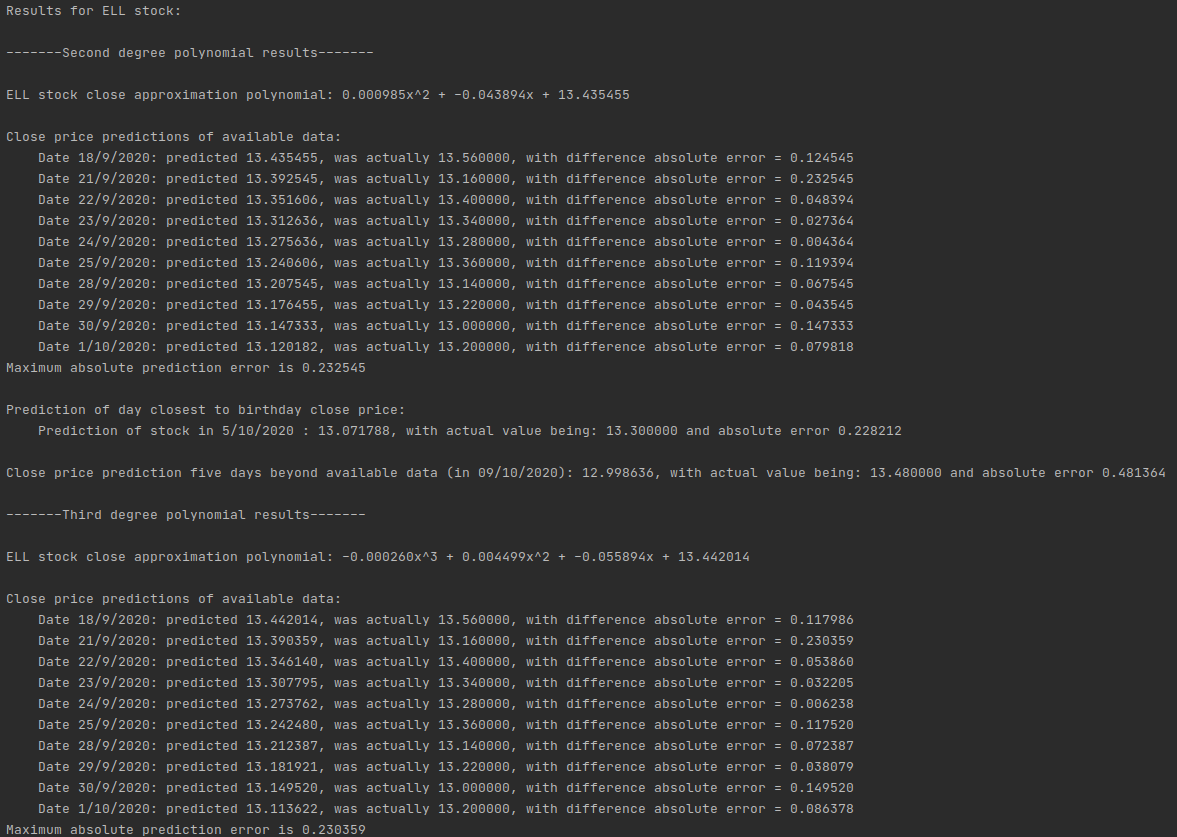
\includegraphics[width=\linewidth]{Exercise7/run_p1.png}\\
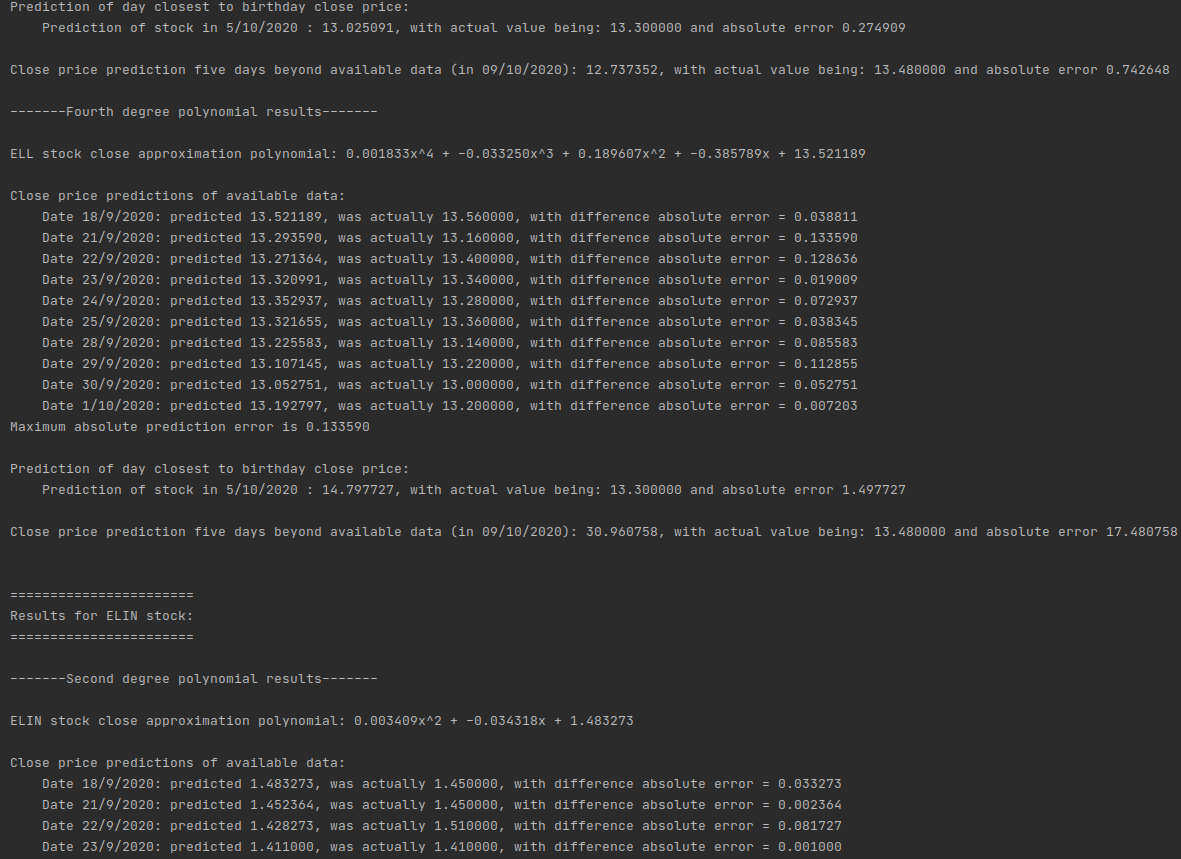
\includegraphics[width=\linewidth]{Exercise7/run_p2.png}\\
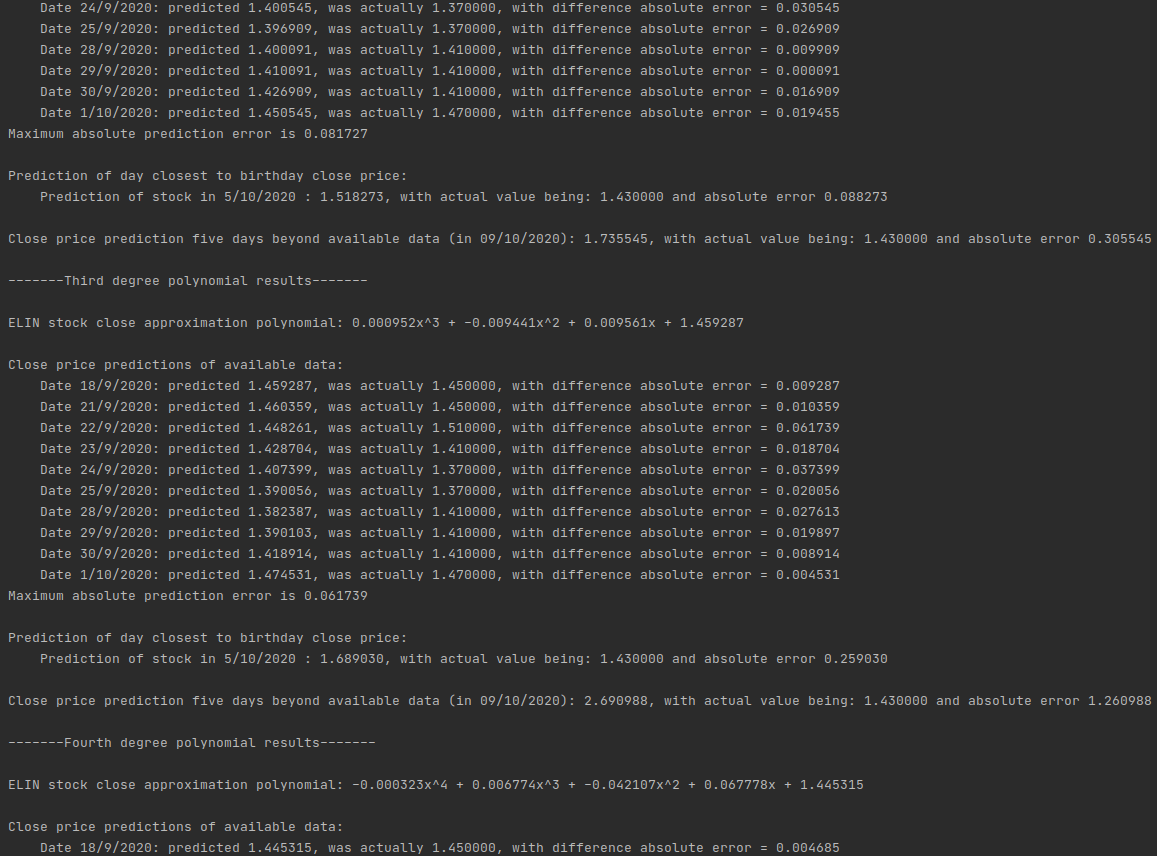
\includegraphics[width=\linewidth]{Exercise7/run_p3.png}\\
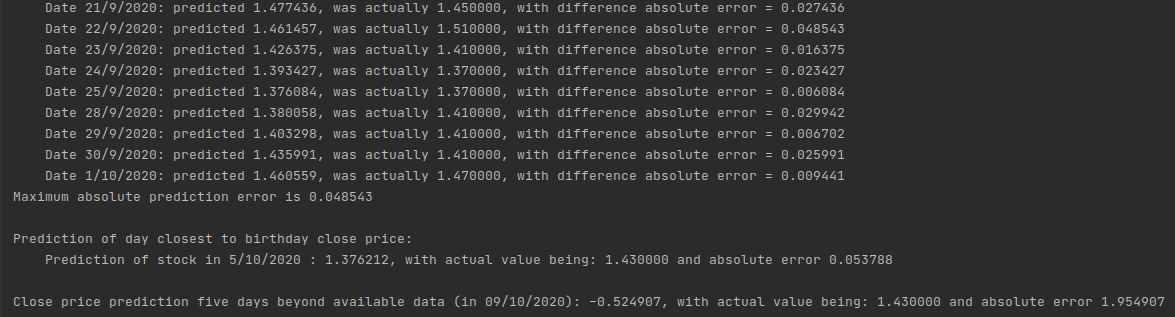
\includegraphics[width=\linewidth]{Exercise7/run_p4.png}\\

\section{Αποτελέσματα}

\subsection{Αποτελέσματα για την μετοχή ΕΛΛ}
Αν εκτελέσουμε τον αρχείο με τον κώδικα (παραπάνω στιγμιότυπα) θα έχουμε τα ακόλουθα αποτελέσματα (με ακρίβεια 6 δεκαδικών ψηφίων) για την μετοχή με σύμβολο ΕΛΛ:\\

\par 
Για πολυώνυμο 2ου βαθμού:\\

Έχω πολυώνυμο 2ου βαθμού που προσεγγίζει την τιμή κλεισίματος της μετοχής: {\lt $0,000985x^2 - 0,043894x + 13,435455$}.\\

Έχω για τις προβλέψεις των δεδομένων που πήρα αρχικά:
\begin{itemize}
    \item Στις 18/9/2020 έχω τιμή μετοχής 13,5600 αλλά πρόβλεψη 13,435455 και απόλυτο σφάλμα προσέγγισης 0,124545
    \item Στις 21/9/2020 έχω τιμή μετοχής 13,1600 αλλά πρόβλεψη 13,392545 και απόλυτο σφάλμα προσέγγισης 0,232545
    \item Στις 22/9/2020 έχω τιμή μετοχής 13,4000 αλλά πρόβλεψη 13,351606 και απόλυτο σφάλμα προσέγγισης 0,048394
    \item Στις 23/9/2020 έχω τιμή μετοχής 13,3400 αλλά πρόβλεψη 13,312636 και απόλυτο σφάλμα προσέγγισης 0,027364
    \item Στις 24/9/2020 έχω τιμή μετοχής 13,2800 αλλά πρόβλεψη 13,275636 και απόλυτο σφάλμα προσέγγισης 0,004364
    \item Στις 25/9/2020 έχω τιμή μετοχής 13,3600 αλλά πρόβλεψη 13,240606 και απόλυτο σφάλμα προσέγγισης 0,119394
    \item Στις 28/9/2020 έχω τιμή μετοχής 13,1400 αλλά πρόβλεψη 13,207545 και απόλυτο σφάλμα προσέγγισης 0,067545
    \item Στις 29/9/2020 έχω τιμή μετοχής 13,2200 αλλά πρόβλεψη 13,176455 και απόλυτο σφάλμα προσέγγισης 0,043545
    \item Στις 30/9/2020 έχω τιμή μετοχής 13,0000 αλλά πρόβλεψη 13,147333 και απόλυτο σφάλμα προσέγγισης 0,147333
    \item Στις 1/10/2020 έχω τιμή μετοχής 13,2000 αλλά πρόβλεψη 13,120182 και απόλυτο σφάλμα προσέγγισης 0,079818
\end{itemize}
Επίσης, έχω μέγιστο σφάλμα προσέγγισης το 0,232545\\

Ακολούθως, έχω πρόβλεψη τιμής κλεισίματος ημέρας μετοχής για την ημέρα κοντινότερη σε αυτή των γενεθλίων μου (5/10) το 13,071788 με πραγματική τιμή να είναι το 13,3000 και το απόλυτο σφάλμα της πρόβλεψης είναι 0,228212\\

Τέλος, η πρόβλεψη για την τιμή κλεισίματος της μετοχής 5 συνεδριάσεων μετά την μέρα των γενεθλίων (στις 09/10/2020) είναι 12,998636 με απόλυτο σφάλμα 0,481364 από την πραγματική 13,4800.\\

\par 
Για πολυώνυμο 3ου βαθμού:\\

Έχω πολυώνυμο 3ου βαθμού που προσεγγίζει την τιμή κλεισίματος της μετοχής: {\lt $-0,000260x^3 + 0,004499x^2 -0,055894x + 13,442014$}.\\


Έχω για τις προβλέψεις των δεδομένων που πήρα αρχικά:
\begin{itemize}
    \item Στις 18/9/2020 έχω τιμή μετοχής 13,5600 αλλά πρόβλεψη 13,442014 και απόλυτο σφάλμα προσέγγισης 0,117986
    \item Στις 21/9/2020 έχω τιμή μετοχής 13,1600 αλλά πρόβλεψη 13,390359 και απόλυτο σφάλμα προσέγγισης 0,230359
    \item Στις 22/9/2020 έχω τιμή μετοχής 13,4000 αλλά πρόβλεψη 13,346140 και απόλυτο σφάλμα προσέγγισης 0,053860
    \item Στις 23/9/2020 έχω τιμή μετοχής 13,3400 αλλά πρόβλεψη 13,307795 και απόλυτο σφάλμα προσέγγισης 0,032205
    \item Στις 24/9/2020 έχω τιμή μετοχής 13,2800 αλλά πρόβλεψη 13,273762 και απόλυτο σφάλμα προσέγγισης 0,006238
    \item Στις 25/9/2020 έχω τιμή μετοχής 13,3600 αλλά πρόβλεψη 13,242480 και απόλυτο σφάλμα προσέγγισης 0,117520
    \item Στις 28/9/2020 έχω τιμή μετοχής 13,1400 αλλά πρόβλεψη 13,212387 και απόλυτο σφάλμα προσέγγισης 0,072387
    \item Στις 29/9/2020 έχω τιμή μετοχής 13,2200 αλλά πρόβλεψη 13,181921 και απόλυτο σφάλμα προσέγγισης 0,038079
    \item Στις 30/9/2020 έχω τιμή μετοχής 13,0000 αλλά πρόβλεψη 13,149520 και απόλυτο σφάλμα προσέγγισης 0,149520
    \item Στις 1/10/2020 έχω τιμή μετοχής 13,2000 αλλά πρόβλεψη 13,113622 και απόλυτο σφάλμα προσέγγισης 0,086378
\end{itemize}
Επίσης, έχω μέγιστο σφάλμα προσέγγισης το 0,230359\\

Ακολούθως, έχω πρόβλεψη τιμής κλεισίματος ημέρας μετοχής για την ημέρα κοντινότερη σε αυτή των γενεθλίων μου (5/10) το 13,025091 με πραγματική τιμή να είναι το 13,3000 και το απόλυτο σφάλμα της πρόβλεψης είναι 0,274909\\

Τέλος, η πρόβλεψη για την τιμή κλεισίματος της μετοχής 5 συνεδριάσεων μετά την μέρα των γενεθλίων (στις 09/10/2020) είναι 12,737352 με απόλυτο σφάλμα 0,742648 από την πραγματική 13,4800.\\

\par 
Για πολυώνυμο 4ου βαθμού:\\

Έχω πολυώνυμο 4ου βαθμού που προσεγγίζει την τιμή κλεισίματος της μετοχής: {\lt $0,001833x^4 -0,033250x^3 + 0,189607x^2 -0,385789x + 13,521189$}.\\

Έχω για τις προβλέψεις των δεδομένων που πήρα αρχικά:
\begin{itemize}
	\item Στις 18/9/2020 έχω τιμή μετοχής 13,5600 αλλά πρόβλεψη 13,521189 και απόλυτο σφάλμα προσέγγισης 0,038811
	\item Στις 21/9/2020 έχω τιμή μετοχής 13,1600 αλλά πρόβλεψη 13,293590 και απόλυτο σφάλμα προσέγγισης 0,133590
	\item Στις 22/9/2020 έχω τιμή μετοχής 13,4000 αλλά πρόβλεψη 13,271364 και απόλυτο σφάλμα προσέγγισης 0,128636
	\item Στις 23/9/2020 έχω τιμή μετοχής 13,3400 αλλά πρόβλεψη 13,320991 και απόλυτο σφάλμα προσέγγισης 0,019009
	\item Στις 24/9/2020 έχω τιμή μετοχής 13,2800 αλλά πρόβλεψη 13,352937 και απόλυτο σφάλμα προσέγγισης 0,072937
	\item Στις 25/9/2020 έχω τιμή μετοχής 13,3600 αλλά πρόβλεψη 13,321655 και απόλυτο σφάλμα προσέγγισης 0,038345
    \item Στις 28/9/2020 έχω τιμή μετοχής 13,1400 αλλά πρόβλεψη 13,225583 και απόλυτο σφάλμα προσέγγισης 0,085583
	\item Στις 29/9/2020 έχω τιμή μετοχής 13,2200 αλλά πρόβλεψη 13,107145 και απόλυτο σφάλμα προσέγγισης 0,112855
	\item Στις 30/9/2020 έχω τιμή μετοχής 13,0000 αλλά πρόβλεψη 13,052751 και απόλυτο σφάλμα προσέγγισης 0,052751
	\item Στις 1/10/2020 έχω τιμή μετοχής 13,2000 αλλά πρόβλεψη 13,192797 και απόλυτο σφάλμα προσέγγισης 0,007203
	\end{itemize}
Επίσης, έχω μέγιστο σφάλμα προσέγγισης το 0,133590\\

Ακολούθως, έχω πρόβλεψη τιμής κλεισίματος ημέρας μετοχής για την ημέρα κοντινότερη σε αυτή των γενεθλίων μου (5/10) το 14,797727 με πραγματική τιμή να είναι το 13,3000 και το απόλυτο σφάλμα της πρόβλεψης είναι 1,497727\\

Τέλος, η πρόβλεψη για την τιμή κλεισίματος της μετοχής 5 συνεδριάσεων μετά την μέρα των γενεθλίων (στις 09/10/2020) είναι 30,960758 με απόλυτο σφάλμα 17,480758 από την πραγματική 13,4800.\\

\par
Επομένως: στα παραπάνω αποτελέσματα συμπεραίνουμε ότι όσο αυξάνει ο βαθμός του πολυωνύμου προσέγγισης, τόσο αυξάνεται η ακρίβεια πρόβλεψης στις γνωστές τιμές.\\
Όμως, στις προβλέψεις τιμών εκτός των γνωστών τιμών (την ημέρα κοντινότερη των γενεθλίων και 5 συνεδριάσεις μετά) η ακρίβεια μειώνεται με την αύξηση του βαθμού του πολυωνύμου, με τον ρυθμό αύξησης του απολύτου σφάλματος να είναι ιδιαίτερα ραγδαίος.

\subsection{Αποτελέσματα για την μετοχή ΕΛΙΝ}
Αν εκτελέσουμε τον αρχείο με τον κώδικα (παραπάνω στιγμιότυπα) θα έχουμε τα ακόλουθα αποτελέσματα (με ακρίβεια 6 δεκαδικών ψηφίων) για την μετοχή με σύμβολο ΕΛΙΝ:\\

\par 
Για πολυώνυμο 2ου βαθμού:\\

Έχω πολυώνυμο 2ου βαθμού που προσεγγίζει την τιμή κλεισίματος της μετοχής: {\lt $0.003409x^2 -0.034318x + 1.483273$}.\\


Έχω για τις προβλέψεις των δεδομένων που πήρα αρχικά:
\begin{itemize}
	\item Στις 18/9/2020 έχω τιμή μετοχής 1,450000 αλλά πρόβλεψη 1,483273 και απόλυτο σφάλμα προσέγγισης 0,033273
	\item Στις 21/9/2020 έχω τιμή μετοχής 1,450000 αλλά πρόβλεψη 1,452364 και απόλυτο σφάλμα προσέγγισης 0,002364
	\item Στις 22/9/2020 έχω τιμή μετοχής 1,510000 αλλά πρόβλεψη 1,428273 και απόλυτο σφάλμα προσέγγισης 0,081727
	\item Στις 23/9/2020 έχω τιμή μετοχής 1,410000 αλλά πρόβλεψη 1,411000 και απόλυτο σφάλμα προσέγγισης 0,001000
	\item Στις 24/9/2020 έχω τιμή μετοχής 1,370000 αλλά πρόβλεψη 1,400545 και απόλυτο σφάλμα προσέγγισης 0,030545
	\item Στις 25/9/2020 έχω τιμή μετοχής 1,370000 αλλά πρόβλεψη 1,396909 και απόλυτο σφάλμα προσέγγισης 0,026909
	\item Στις 28/9/2020 έχω τιμή μετοχής 1,410000 αλλά πρόβλεψη 1,400091 και απόλυτο σφάλμα προσέγγισης 0,009909
	\item Στις 29/9/2020 έχω τιμή μετοχής 1,410000 αλλά πρόβλεψη 1,410091 και απόλυτο σφάλμα προσέγγισης 0,000091
	\item Στις 30/9/2020 έχω τιμή μετοχής 1,410000 αλλά πρόβλεψη 1,426909 και απόλυτο σφάλμα προσέγγισης 0,016909
	\item Στις 1/10/2020 έχω τιμή μετοχής 1,470000 αλλά πρόβλεψη 1,450545 και απόλυτο σφάλμα προσέγγισης 0,019455
\end{itemize}
Επίσης, έχω μέγιστο σφάλμα προσέγγισης το 0,081727\\

Ακολούθως, έχω πρόβλεψη τιμής κλεισίματος ημέρας μετοχής για την ημέρα κοντινότερη σε αυτή των γενεθλίων μου (5/10) το 1,518273 με πραγματική τιμή να είναι το 1,4300 και το απόλυτο σφάλμα της πρόβλεψης είναι 0,088273\\

Τέλος, η πρόβλεψη για την τιμή κλεισίματος της μετοχής 5 συνεδριάσεων μετά την μέρα των γενεθλίων (στις 09/10/2020) είναι 1,735545 με απόλυτο σφάλμα 0,305545 από την πραγματική 1,4300.\\

\par 
Για πολυώνυμο 3ου βαθμού:\\

Έχω πολυώνυμο 3ου βαθμού που προσεγγίζει την τιμή κλεισίματος της μετοχής: {\lt $0.000952x^3 -0.009441x^2 + 0.009561x + 1.459287$}.\\


Έχω για τις προβλέψεις των δεδομένων που πήρα αρχικά:
\begin{itemize}
	\item Στις 18/9/2020 έχω τιμή μετοχής 1,450000 αλλά πρόβλεψη 1,459287 και απόλυτο σφάλμα προσέγγισης 0,009287
	\item Στις 21/9/2020 έχω τιμή μετοχής 1,450000 αλλά πρόβλεψη 1,460359 και απόλυτο σφάλμα προσέγγισης 0,010359
	\item Στις 22/9/2020 έχω τιμή μετοχής 1,510000 αλλά πρόβλεψη 1,448261 και απόλυτο σφάλμα προσέγγισης 0,061739
	\item Στις 23/9/2020 έχω τιμή μετοχής 1,410000 αλλά πρόβλεψη 1,428704 και απόλυτο σφάλμα προσέγγισης 0,018704
	\item Στις 24/9/2020 έχω τιμή μετοχής 1,370000 αλλά πρόβλεψη 1,407399 και απόλυτο σφάλμα προσέγγισης 0,037399
	\item Στις 25/9/2020 έχω τιμή μετοχής 1,370000 αλλά πρόβλεψη 1,390056 και απόλυτο σφάλμα προσέγγισης 0,020056
	\item Στις 28/9/2020 έχω τιμή μετοχής 1,410000 αλλά πρόβλεψη 1,382387 και απόλυτο σφάλμα προσέγγισης 0,027613
	\item Στις 29/9/2020 έχω τιμή μετοχής 1,410000 αλλά πρόβλεψη 1,390103 και απόλυτο σφάλμα προσέγγισης 0,019897
	\item Στις 30/9/2020 έχω τιμή μετοχής 1,410000 αλλά πρόβλεψη 1,418914 και απόλυτο σφάλμα προσέγγισης 0,008914
	\item Στις 1/10/2020 έχω τιμή μετοχής 1,470000 αλλά πρόβλεψη 1,474531 και απόλυτο σφάλμα προσέγγισης 0,004531
\end{itemize}
Επίσης, έχω μέγιστο σφάλμα προσέγγισης το 0,061739\\

Ακολούθως, έχω πρόβλεψη τιμής κλεισίματος ημέρας μετοχής για την ημέρα κοντινότερη σε αυτή των γενεθλίων μου (5/10) το 1,689030 με πραγματική τιμή να είναι το 1,4300 και το απόλυτο σφάλμα της πρόβλεψης είναι 0,259030\\

Τέλος, η πρόβλεψη για την τιμή κλεισίματος της μετοχής 5 συνεδριάσεων μετά την μέρα των γενεθλίων (στις 09/10/2020) είναι 2,690988 με απόλυτο σφάλμα 1,260988 από την πραγματική 1,4300.\\

\par 
Για πολυώνυμο 4ου βαθμού:\\

Έχω πολυώνυμο 4ου βαθμού που προσεγγίζει την τιμή κλεισίματος της μετοχής: {\lt $-0.000323x^4 + 0.006774x^3 -0.042107x^2 + 0.067778x + 1.445315$}.\\


Έχω για τις προβλέψεις των δεδομένων που πήρα αρχικά:
\begin{itemize}
	\item Στις 18/9/2020 έχω τιμή μετοχής 1,450000 αλλά πρόβλεψη 1,445315 και απόλυτο σφάλμα προσέγγισης 0,004685
	\item Στις 21/9/2020 έχω τιμή μετοχής 1,450000 αλλά πρόβλεψη 1,477436 και απόλυτο σφάλμα προσέγγισης 0,027436
	\item Στις 22/9/2020 έχω τιμή μετοχής 1,510000 αλλά πρόβλεψη 1,461457 και απόλυτο σφάλμα προσέγγισης 0,048543
	\item Στις 23/9/2020 έχω τιμή μετοχής 1,410000 αλλά πρόβλεψη 1,426375 και απόλυτο σφάλμα προσέγγισης 0,016375
	\item Στις 24/9/2020 έχω τιμή μετοχής 1,370000 αλλά πρόβλεψη 1,393427 και απόλυτο σφάλμα προσέγγισης 0,023427
	\item Στις 25/9/2020 έχω τιμή μετοχής 1,370000 αλλά πρόβλεψη 1,376084 και απόλυτο σφάλμα προσέγγισης 0,006084
	\item Στις 28/9/2020 έχω τιμή μετοχής 1,410000 αλλά πρόβλεψη 1,380058 και απόλυτο σφάλμα προσέγγισης 0,029942
	\item Στις 29/9/2020 έχω τιμή μετοχής 1,410000 αλλά πρόβλεψη 1,403298 και απόλυτο σφάλμα προσέγγισης 0,006702
	\item Στις 30/9/2020 έχω τιμή μετοχής 1,410000 αλλά πρόβλεψη 1,435991 και απόλυτο σφάλμα προσέγγισης 0,025991
	\item Στις 1/10/2020 έχω τιμή μετοχής 1,470000 αλλά πρόβλεψη 1,460559 και απόλυτο σφάλμα προσέγγισης 0,009441
	\end{itemize}
Επίσης, έχω μέγιστο σφάλμα προσέγγισης το 0,048543\\

Ακολούθως, έχω πρόβλεψη τιμής κλεισίματος ημέρας μετοχής για την ημέρα κοντινότερη σε αυτή των γενεθλίων μου (5/10) το 1,376212 με πραγματική τιμή να είναι το 1,4300 και το απόλυτο σφάλμα της πρόβλεψης είναι 0,053788\\

Τέλος, η πρόβλεψη για την τιμή κλεισίματος της μετοχής 5 συνεδριάσεων μετά την μέρα των γενεθλίων (στις 09/10/2020) είναι -0,524907 (που προφανώς δεν πρέπει να ορίζεται αρνητική τιμή μετοχής) με απόλυτο σφάλμα 1,954907 από την πραγματική 1,4300.\\

\par
Επομένως: στα παραπάνω αποτελέσματα συμπεραίνουμε ότι όσο αυξάνει ο βαθμός του πολυωνύμου προσέγγισης, τόσο αυξάνεται η ακρίβεια πρόβλεψης στις γνωστές τιμές.\\
Όμως, στην πρόβλεψη τιμής στην ημέρα κοντινότερη των γενεθλίων παρατηρούμε μία σημαντική αύξηση του απολύτου σφάλματος από <<μετάβαση>> του πολυωνύμου από 2ο σε 3ο βαθμό και μείωση του απολύτου σφάλματος στην <<μετάβαση>> από 3ο σε 4ο βαθμό πολυωνύμου.\\
Τέλος, στην πρόβλεψη τιμής 5 μέρες μετά από την ημέρα των γενεθλίων η ακρίβεια μειώνεται, με την αύξηση του βαθμού του πολυωνύμου.
\end{document}